\documentclass[border=4pt]{standalone}
\usepackage{tikz}
\usetikzlibrary{calc}
\definecolor{orangeText}{HTML}{E3A063}
\definecolor{orangeDim}{HTML}{A87A4E}
\begin{document}
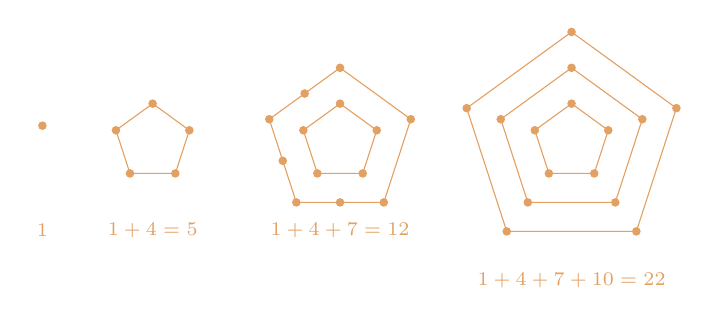
\begin{tikzpicture}[color=orangeText, scale=0.7,dot/.style={circle,fill,inner sep=1.1pt}]
  % (a) 1 point
  \node[dot] at (0,0.3) {};
  \node at (0,-1.6) {\scriptsize 1};
  % (b) pentagon 5
  \begin{scope}[xshift=2cm]
    \foreach \i in {0,...,4} {\coordinate (a\i) at ({90+72*\i}:0.7);}
    \draw (a0)--(a1)--(a2)--(a3)--(a4)--cycle;
    \foreach \i in {0,...,4} \node[dot] at (a\i) {};
    \node at (0,-1.6) {\scriptsize $1+4=5$};
  \end{scope}
  % (c) 12
  \begin{scope}[xshift=5.4cm]
    \foreach \i in {0,...,4} {\coordinate (b\i) at ({90+72*\i}:1.35);}
    \foreach \i in {0,...,4} {\coordinate (c\i) at ({90+72*\i}:0.7);}
    \draw (b0)--(b1)--(b2)--(b3)--(b4)--cycle;
    \draw (c0)--(c1)--(c2)--(c3)--(c4)--cycle;
    \foreach \i in {0,...,4} {\node[dot] at (b\i) {}; \node[dot] at (c\i) {};}
    \node[dot] at ($(b0)!0.5!(b1)$) {}; \node[dot] at ($(b1)!0.5!(b2)$) {};
    \node[dot] at ($(b2)!0.5!(b3)$) {};
    \node at (0,-1.6) {\scriptsize $1+4+7=12$};
  \end{scope}
  % (d) 22
  \begin{scope}[xshift=9.6cm]
    \foreach \i in {0,...,4} {\coordinate (d\i) at ({90+72*\i}:2.0);}
    \foreach \i in {0,...,4} {\coordinate (e\i) at ({90+72*\i}:1.35);}
    \foreach \i in {0,...,4} {\coordinate (f\i) at ({90+72*\i}:0.7);}
    \draw (d0)--(d1)--(d2)--(d3)--(d4)--cycle;
    \draw (e0)--(e1)--(e2)--(e3)--(e4)--cycle;
    \draw (f0)--(f1)--(f2)--(f3)--(f4)--cycle;
    \foreach \i in {0,...,4} {\node[dot] at (d\i) {}; \node[dot] at (e\i) {}; \node[dot] at (f\i) {};}
    \node at (0,-2.5) {\scriptsize $1+4+7+10=22$};
  \end{scope}
\end{tikzpicture}
\end{document}
